% Shared preamble for both journal versions. Keep journal-specific settings
% in main-enb.tex / main-jbps.tex.
\usepackage[T1]{fontenc}
\usepackage[utf8]{inputenc}
\usepackage{lmodern}
\usepackage[british]{babel}
\usepackage{amsmath,amssymb}
\usepackage{graphicx}
\usepackage{booktabs}
\usepackage{tabularx}
\usepackage{array}
\usepackage{longtable}
\usepackage{siunitx}
\usepackage{textcomp}
\usepackage{newunicodechar}
\newunicodechar{°}{\textdegree}
\newunicodechar{²}{\textsuperscript{2}}
\newunicodechar{●}{\ensuremath{\bullet}}
\newunicodechar{−}{\ensuremath{-}}
\newunicodechar{±}{\ensuremath{\pm}}
\newunicodechar{·}{\ensuremath{\cdot}}
\newunicodechar{×}{\ensuremath{\times}}
\newunicodechar{≈}{\ensuremath{\approx}}
\usepackage{xcolor}
\usepackage{caption}
\usepackage[hidelinks]{hyperref}
\usepackage{xurl}

\sisetup{detect-all}
\setlength{\emergencystretch}{3em}
\renewcommand{\arraystretch}{1.15}
\newcolumntype{L}[1]{>{\raggedright\arraybackslash}p{#1}}
\newcolumntype{Y}{>{\raggedright\arraybackslash}X}

% Figures: drop updated files into figures/ with the same names.
% \includegraphics picks .pdf first, then .png.
\graphicspath{{figures/}}
\DeclareGraphicsExtensions{.pdf,.png,.jpg}

% Shows a framed placeholder when a figure file is not there yet,
% so the paper always compiles.
\newcommand{\paperfigure}[2][width=\linewidth]{%
  \IfFileExists{figures/#2.pdf}{\includegraphics[#1]{#2}}{%
  \IfFileExists{figures/#2.png}{\includegraphics[#1]{#2}}{%
  \fbox{\parbox[c][5cm][c]{0.9\linewidth}{\centering Figure file \texttt{figures/#2} not yet added}}}}}

\newcommand{\papertitle}{How much does filling gaps in weather data change building energy results? A hide-and-refill test}
\newcommand{\correspondingemail}{sanjay.somanath@chalmers.se}

\newcommand{\graphicalabstractslot}{%
  \IfFileExists{figures/graphical_abstract.pdf}{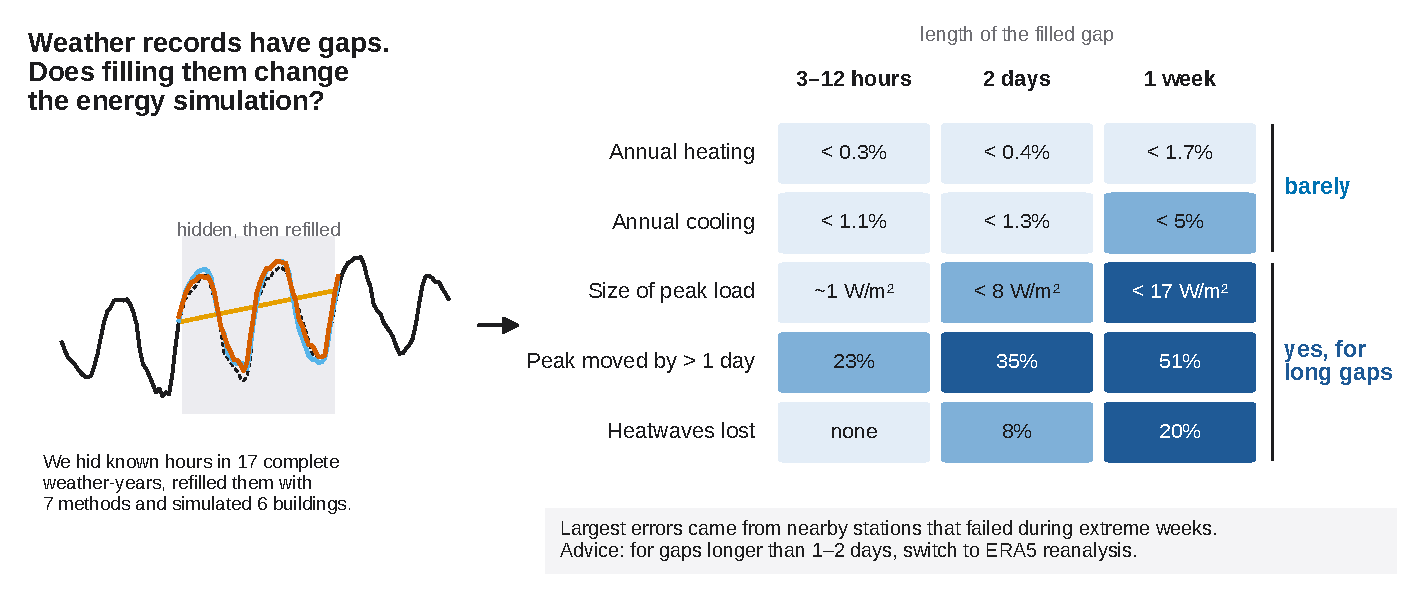
\includegraphics[width=\linewidth]{graphical_abstract}}{%
  \IfFileExists{figures/graphical_abstract.png}{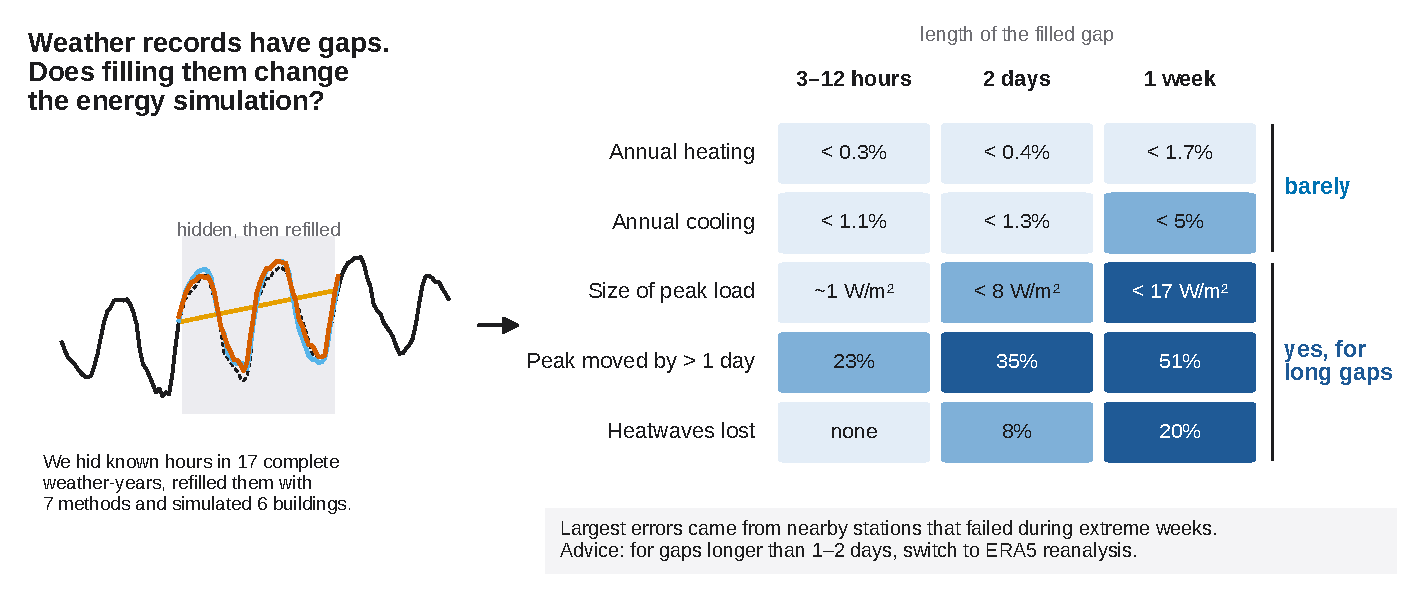
\includegraphics[width=\linewidth]{graphical_abstract}}{%
  \fbox{\parbox[c][6cm][c]{0.9\linewidth}{\centering Graphical abstract: add \texttt{figures/graphical\_abstract.pdf}\\(Elsevier: 1328 $\times$ 531 px or larger, readable at 5 $\times$ 13 cm)}}}}}
